% LaTex source code
% File: "diss.tex"
% Created: "Ter, 08 Abr 2014 14:27:10 +0200 (kassick)"
% Updated: "Seg, 13 Out 2014 12:29:29 -0300 (kassick)"
% $Id$
% Copyright (C) 2014, Rodrigo Virote Kassick <rvkassick@inf.ufrgs.br> 
% exemplo genérico de uso da classe iiufrgs.cls baseado em
% $Id: iiufrgs.tex,v 1.1.1.1 2005/01/18 23:54:42 avila Exp $
%
% This is an example file and is hereby explicitly put in the
% public domain.
%


% Um tipo específico de monografia pode ser informado como parâmetro opcional:
% 
%\documentclass[tese]{iiufrgs}
%\documentclass[tc-cic]{iiufrgs}
%\documentclass[tc-ecp]{iiufrgs}
%...
%@TODO: Atualizar depois que todos os .def tenham sido criados

\documentclass[diss,ppgc,openright,english]{iiufrgs}

% Outras Opções:
%   * english    -- para textos em inglês
%   * openright  -- Força início de capítulos em páginas ímpares (padrão da
%                   biblioteca)
%   * oneside    -- Desliga frente-e-verso
%   * nominatalocal -- Lê os dados da nominata do arquivo nominatalocal.def


% Estamos no século 21. Use unicode.
%\usepackage{ucs}
\usepackage{subfigure}
\usepackage[utf8]{inputenc}

% @TODO: t1 fontenc ainda é necessário? Se sim, @TODO: Mover t1 fontenc para a
% classe
\usepackage[T1]{fontenc}

% @TODO: Qual dessas é o padrão da biblioteca ?
\usepackage{times}
% \usepackage{palatino}

% Alguns pacotes úteis
% \usepackage{url}                % comando \url{} para formatar urls corretamente
\usepackage{graphicx}           % suporte a vários formatos gráficos
%\usepackage{mathptmx}           % p/ usar fonte Adobe Times nas fórmulas
%\usepackage{amsmath}            % Extensões da American Mathematical Society
%\usepackage{array}              % Formatação de fórmulas
%\usepackage{color}              % Definições de cores
%\usepackage{hhline}
%\usepackage{tabularx}           % permite colunas tipo parágrafo que expandem pro espaço disponível
%\usepackage{longtable}          % longtable e xtab dão suporte a tabelas muito 
%\usepackage{xtab}               % longas (mais de uma página). Escolha uma
%\usepackage{multirow}           % Permite mesclar linhas de um tabular
%\usepackage{calc}               % Para operar counters
%\usepackage{ifthen}             % Útil para construir comandos de latex
%\usepackage{xspace}             % Insere um espaço SSE o próximo caracter nâo for de pontuação.

\usepackage[alf,abnt-emphasize=bf]{abntex2cite}	% pacote para usar citações abnt




%
% Informações gerais
%
\title{Um Exemplo de Monografia do Instituto de Informática da UFRGS}

\author{Flaumann}{Fritz Gutenberg}
% alguns documentos podem ter varios autores:
%\author{Flaumann}{Frida Gutenberg}
%\author{Flaumann}{Klaus Gutenberg}

% orientador e co-orientador são opcionais (não diga isso pra eles :))
\advisor[Prof.~Dr.]{Lamport}{Leslie}
%\coadvisor[Prof.~Dr.]{Knuth}{Donald Ervin}

% a data deve ser a da defesa; se nao especificada, são gerados
% mes e ano correntes
%\date{maio}{2001}

% o nome do curso pode ser redefinido (ex. para TCs)
%\course{Curso de Especialização em Cachaça}

% o local de realização do trabalho pode ser especificado (ex. para TCs)
% com o comando \location:
%\location{Itaquaquecetuba}{SP}

% itens individuais da nominata podem ser redefinidos com os comandos
% abaixo:
% \renewcommand{\nominataReit}{Prof\textsuperscript{a}.~Wrana Maria Panizzi}
% \renewcommand{\nominataReitname}{Reitora}
% \renewcommand{\nominataPRE}{Prof.~Jos{\'e} Carlos Ferraz Hennemann}
% \renewcommand{\nominataPREname}{Pr{\'o}-Reitor de Ensino}
% \renewcommand{\nominataPRAPG}{Prof\textsuperscript{a}.~Joc{\'e}lia Grazia}
% \renewcommand{\nominataPRAPGname}{Pr{\'o}-Reitora Adjunta de P{\'o}s-Gradua{\c{c}}{\~a}o}
% \renewcommand{\nominataDir}{Prof.~Philippe Olivier Alexandre Navaux}
% \renewcommand{\nominataDirname}{Diretor do Instituto de Inform{\'a}tica}
% \renewcommand{\nominataCoord}{Prof.~Carlos Alberto Heuser}
% \renewcommand{\nominataCoordname}{Coordenador do PPGC}
% \renewcommand{\nominataBibchefe}{Beatriz Regina Bastos Haro}
% \renewcommand{\nominataBibchefename}{Bibliotec{\'a}ria-chefe do Instituto de Inform{\'a}tica}
% \renewcommand{\nominataChefeINA}{Prof.~Jos{\'e} Valdeni de Lima}
% \renewcommand{\nominataChefeINAname}{Chefe do \deptINA}
% \renewcommand{\nominataChefeINT}{Prof.~Leila Ribeiro}
% \renewcommand{\nominataChefeINTname}{Chefe do \deptINT}

% A seguir são apresentados comandos específicos para alguns
% tipos de documentos.

% Relatório de Pesquisa [rp]:
% \rp{123}             % numero do rp
% \financ{CNPq, CAPES} % orgaos financiadores

% Trabalho Individual [ti]:
% \ti{123}     % numero do TI
% \ti[II]{456} % no caso de ser o segundo TI

% Trabalho de Conclusão [tc]:
% além de definir explicitamente o nome do curso (\course) e o local
% de realização (\location), é necessário redefinir a nominata,
% pois as informações necessárias dependem do curso. Ex.:
%\renewcommand{\nominata}{
%        UNIVERSIDADE FEDERAL DO RIO GRANDE DO SUL\\
%        Reitora: Prof\textsuperscript{a}.~Wrana Maria Panizzi\\
%        Pró-Reitor de Ensino: Prof.~José Carlos Ferraz Hennemann\\
%        Diretor do Instituto de Informática: Prof.~Philippe Olivier Alexandre Navaux\\
%        Coordenador do curso: Prof.~Seu Creysson\\
%        Bibliotecária-chefe do Instituto de Informática: Beatriz Regina Bastos Haro
%}

% Monografias de Especialização [espec]:
% \espec{Redes e Sistemas Distribuídos}      % nome do curso
% \coord[Profa.~Dra.]{Weber}{Taisy da Silva} % coordenador do curso
% \dept{INA}                                 % departamento relacionado

%
% palavras-chave
% iniciar todas com letras minúsculas, exceto no caso de abreviaturas
%
\keyword{formatação eletrônica de documentos}
\keyword{\LaTeX}
\keyword{ABNT}
\keyword{UFRGS}

%
% inicio do documento
%
\begin{document}

% folha de rosto
% às vezes é necessário redefinir algum comando logo antes de produzir
% a folha de rosto:
% \renewcommand{\coordname}{Coordenadora do Curso}
\maketitle

% dedicatoria
\clearpage
\begin{flushright}
\mbox{}\vfill
{\sffamily\itshape
``If I have seen farther than others,\\
it is because I stood on the shoulders of giants.''\\}
--- \textsc{Sir~Isaac Newton}

and me, of course.

\end{flushright}

% agradecimentos
\chapter*{Agradecimentos}
Agradeço ao \LaTeX\ por não ter vírus de macro\ldots

% sumario
\tableofcontents

% lista de abreviaturas e siglas
% o parametro deve ser a abreviatura mais longa
\begin{listofabbrv}{SPMD}
        \item[SMP] Symmetric Multi-Processor
        \item[NUMA] Non-Uniform Memory Access
        \item[SIMD] Single Instruction Multiple Data
        \item[SPMD] Single Program Multiple Data
        \item[ABNT] Associação Brasileira de Normas Técnicas
\end{listofabbrv}

% idem para a lista de símbolos
%\begin{listofsymbols}{$\alpha\beta\pi\omega$}
%       \item[$\sum{\frac{a}{b}}$] Somatório do produtório
%       \item[$\alpha\beta\pi\omega$] Fator de inconstância do resultado
%\end{listofsymbols}

% lista de figuras
\listoffigures

% lista de tabelas
%\listoftables

% resumo na língua do documento
\begin{abstract}
Este documento é um exemplo de como formatar documentos para o
Instituto de Informática da UFRGS usando as classes \LaTeX\
disponibilizadas pelo UTUG\@. Ao mesmo tempo, pode servir de consulta
para comandos mais genéricos. \emph{O texto do resumo não deve
conter mais do que 500 palavras.}
\end{abstract}

% resumo na outra língua
% como parametros devem ser passados o titulo e as palavras-chave
% na outra língua, separadas por vírgulas
\begin{englishabstract}{Using \LaTeX\ to Prepare Documents at II/UFRGS}{Electronic document preparation, \LaTeX, ABNT, UFRGS}
This document is an example on how to prepare documents at II/UFRGS
using the \LaTeX\ classes provided by the UTUG\@. At the same time, it
may serve as a guide for general-purpose commands. \emph{The text in
the abstract should not contain more than 500~words.}
\end{englishabstract}

% aqui comeca o texto propriamente dito

% introducao
\chapter{Introdução}

No início dos tempos, Donald E. Knuth criou o \TeX. Algum tempo depois, Leslie Lamport criou o \LaTeX. Graças a eles, não somos obrigados a usar o Word nem o StarOffice.

\section{Figuras e tabelas}

Esta seção faz referência às Figuras~\ref{fig:ex1} e~\ref{fig:ex2}, a título de exemplo. A primeira representa o caso mais comum, onde a figura propriamente dita é importada de um arquivo \texttt{.eps} (aplicativos como \emph{xfig} e \emph{dia} estão entre os mais usados para gerar figuras no formato \texttt{.eps}). A segunda exemplifica o uso do environment \texttt{picture}, para desenhar usando o próprio~\LaTeX.


\begin{figure}
    \subfigure[a]{aaa}
        \centerline{
            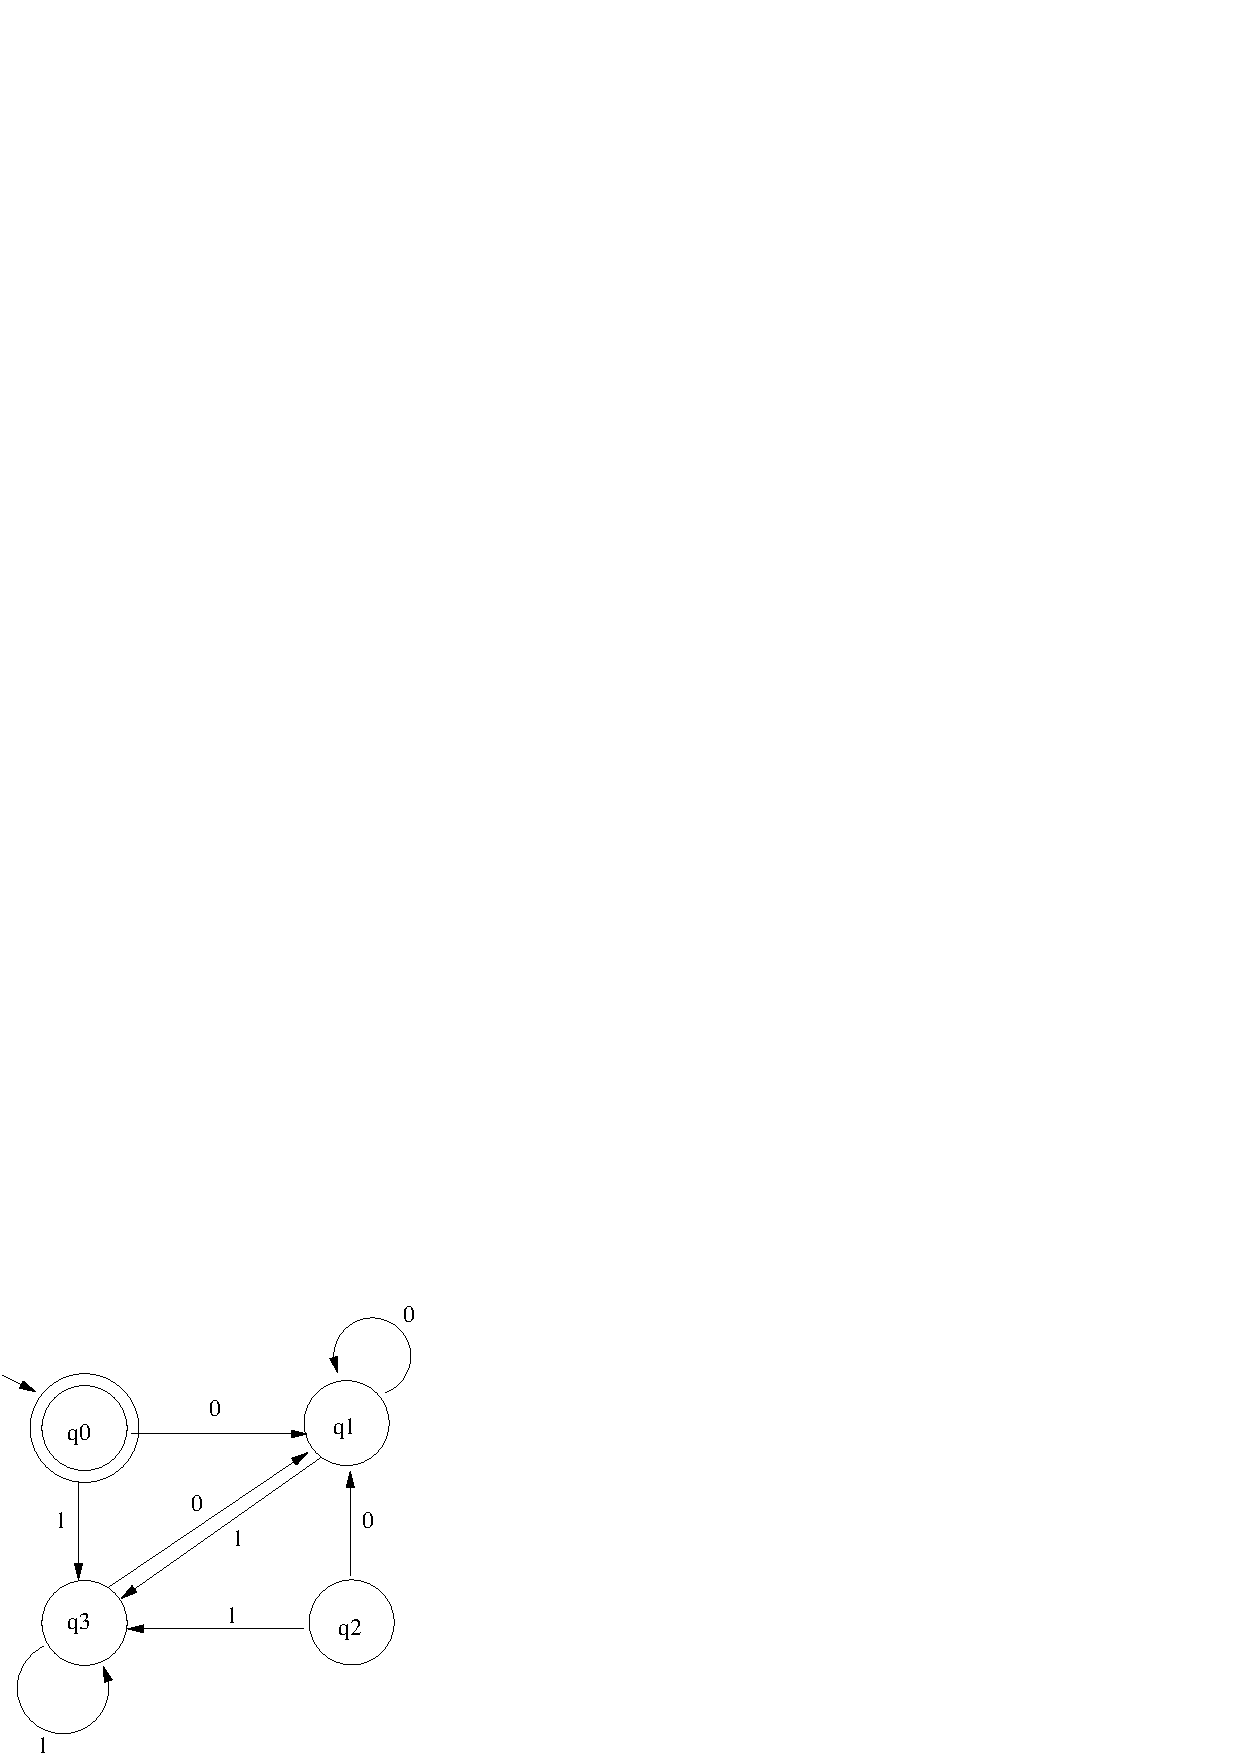
\includegraphics[width=8em]{fig.pdf}
        }
        \caption{Exemplo de figura importada de um arquivo \texttt{.svg} e também exemplo de caption muito grande que ocupa mais de uma linha na Lista~de~Figuras}
        \label{fig:ex1}
\end{figure}


% o `[h]' abaixo é um parâmetro opcional que sugere que o LaTeX coloque a
% figura exatamente neste ponto do texto. Somente preocupe-se com esse tipo
% de formatação quando o texto estiver completamente pronto (uma frase a mais
% pode fazer o LaTeX mudar completamente de idéia sobre onde colocar as
% figuras e tabelas)
%\begin{figure}[h]
\begin{figure}
        \begin{center}
        \setlength{\unitlength}{.1em}
        \begin{picture}(100,100)
                \put(20,20){\circle{20}}
                \put(20,20){\small\makebox(0,0){a}}
                \put(80,80){\circle{20}}
                \put(80,80){\small\makebox(0,0){b}}
                \put(28,28){\vector(1,1){44}}
        \end{picture}
        \end{center}
        \caption{Exemplo de figura desenhada com o environment \texttt{picture}.}
        \label{fig:ex2}
\end{figure}

Tabelas são construídas com praticamente os mesmos comandos. Lembre-se, porém, que o caption das tabelas deve ir em cima.

\subsection{Classificação dos etc.}

O formato adotado pela ABNT prevê apenas três níveis (capítulo, seção e subseção). Assim, \texttt{\char'134subsubsection} não é aconselhado.

\section{Sobre as referências bibliográficas}

A classe \emph{iiufrgs} faz uso do pacote \emph{abnTeX2} com algumas alterações
feitas por Sandro Rama Fiorini. Culpe ele se algo der errado. Agradeça a ele
pelo que der certo. As modificações dão uma camada de tinta NATBIB-style,
já que o abntex2 usa uns comandos de citação feitos para alienívenas de 5 braços 
wtf. Exemplos de citação:

\begin{itemize}
    \item \emph{cite}: \cite{Adams2009Conceptual};
    \item \emph{citep}:\citep{Adams2009Conceptual};
    \item \emph{citet}: \citet{Adams2009Conceptual}
    \item \emph{citen or citenum}: \citen{Adams2009Conceptual}
    \item \emph{citeyearpar} \citeyearpar{Adams2009Conceptual};
\end{itemize}

O estilo abnt fornecido antigamente pelo UTUG não é mais recomendado, pois não
produz saída de acordo com as exigências da biblioteca.


% e aqui vai a parte principal
%
% \chapter{Estado da arte}
% \chapter{Mais estado da arte}
% \chapter{A minha contribuição}
% \chapter{Prova de que a minha contribuição é válida}
% \chapter{Conclusão}


% Use o estilo bibliográfico fornecido pelo modelo
\bibliographystyle{abntex2-alf}
\bibliography{biblio}



\end{document}
